\chapter{Background}
%In this chapter, all background necessary to understand the thesis are introduced. The level of detail is such that a colleague with similar background (no specialist!) is capable of understanding the contribution and impact of the thesis. A discussion of state-of-the-art solutions (e.g. literature research) is often helpful. Problems of the state-of-the-art are typically discussed and the contribution of the thesis is introduced in detail.

The chapter discusses the basic terminologies and approach used in this internship, followed by the
research question of this internship, the related work and various existing tools were found to be suitable or unsuitable to achieve the goals.

%\section{Content}
%Probably explain about the requirements of industrial communication, Time slotted channel hopping, Time synchronization, Super frame concept probably.

Industrial domain has opted wireless sensor networks over traditional wired communication due to several attractive features of IWSN's such as self-organization, rapid deployment, flexibility.  the explosive growth that has occurred in the use of wireless sensor networks in a variety of applications. As wireless technology can reduce costs, increase productivity, and ease maintenance. However the advantages come with some challenges which needs to addressed.

The major technical challenges involved for the deployment of IWSNs are outlined as follows.

\textbf{Resource constraints:} The wireless nodes are constrained in terms of memory, power and processing power.

\textbf{Dynamic topologies:} Routing between the central hub and leaf nodes is done through hop by hop, so if one node fails in the path network should be able to find another route to communicate with central node.(Not applicable for single hop)

\textbf{Latency requirements:} The wide variety of use cases conceived as possibility on IWSNs will have different QoS requirements and specifications. The QoS provided by IWSNs refers to the accuracy between the data reported central hub(industrial controller) and what is actually happening in the plant. In addition, since sensor data are typically time-sensitive, e.g., receiving the sensor readings on time in a control loop, it is important to receive the data at the sink in a timely manner. Data with long latency due to processing or communication may be outdated and lead to wrong decisions in the industrial controller.

\textbf{Packet errors and variable-link capacity:} Compared to wired networks, in IWSNs, the attainable capacity of each wireless link depends on the interference level perceived at the receiver, and high bit error rates (BER=10\textsuperscript{-2}-10\textsuperscript{-6}) are observed in communication. In addition, wireless links exhibit widely varying characteristics over time and space due to obstructions and noisy environment. Thus, capacity and delay attainable at each link are location-dependent and vary continuously, making QoS provisioning a challenging task.

\textbf{Integration with Internet and other networks:} It is of fundamental importance for the commercial development of IWSNs to provide services that allow the querying of the network to retrieve useful information from anywhere and at any time. For this reason, the IWSNs should be remotely accessible from the Internet and, hence, need to be integrated with the Internet Protocol (IP) architecture.

\section{OpenWSN Stack}
OpenWSN is open source internet of things stack based on highly reliable time slotted channel hopping based MAC layer protocol 802.15.4e. The stack implements RPL procotol for upward routing and source routing for downward traffic. The stack uses 6LowPAN. 6LowPAN is an IPv6 over low power wireless personal area networks it defines the encapsulation and header compression mechanism for sending and receiving IPv6 packets over 802.15.4 networks.

\begin{figure}[H]
	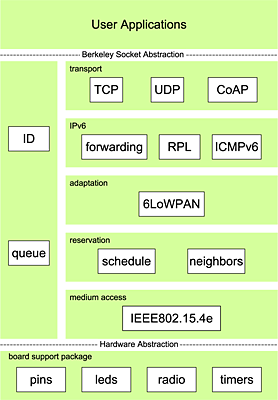
\includegraphics[scale=1,width=0.3\linewidth,center]{openwsn.png}
	\caption{OpenWSN stack\cite{ETT:ETT2558}}
	\label{fig:fig1}
\end{figure}
 
\section{TSCH}
Reliability and deterministic behavior is required in industrial communication with low power consumption, since nodes are running with scavenged or battery power. TSCH is medium access mechanism inspired from WirelessHART and ISA100.11a. 
TSCH(Time slotted channel hopping)provides both low power and high reliability. In TSCH mechanism nodes in the network are time synchronized with the super frame and cells are allocated between the nodes, Nodes have to turn the radio on only during their slot otherwise radio will be turned off. This method in addition to saving the power reduces packet collisions since only one node can transmit packet in a particular slot. 6tisch is an implementation of TSCH over IPv6.

\section{LLDN}
Factory automation applications require large number of nodes to observe and control production. Nodes need to collect data from robots, portable machine tools, such as milling machines. This applications mostly require high determinism,reliability and low latency. LLDN(Low Latency Deterministic Network) standard of IEEE considers latency as main QoS element.

LLDN supports only star topology because of low latency requirements, LLDN superframe is a time division multiple access(TDMA) scheme. LLDN nodes only synchronized beacons frames, Sychronization with acks is not possible since acks are removed to reduce latency.

\section{Problem description}
OpenWSN is an opensource implementation of a 6tisch standard coupled with internet of things standards such as 6LoWPAN,RPL and CoAP allows low power ultra reliable communication, However design is not optimal for low latency communication and also out of the box it is very difficult to use OpenWSN for evaluating capillary networks for latency and reliability. In this research internship, The task is to improve the existing OpenWSN stack to use it for evaluating latency bottlenecks and also to set up low latency deterministic network. In the internship new modules,API's are added and existing implementations are improved for achieving the desired goal.

%and implementation becoming popular research environments, However it is not designed for evaluatby keeping industrial communication in mind. because evaluations are not done for latency and reliability requirements of the industrial networks. 

